% !TEX TS-program = lualatex
%\documentclass[handout]{beamer}
\documentclass{beamer}
\input{../common/misomva}
\begin{document}
% Topic-specific title slide

\newcommand{\topictitle}{Similarity Graphs Introduction}

\newcommand{\topicsubtitle}{From Data to Graphs}
\newcommand{\misoclasstinytitleslide}{Partially based on material by:  Andreas Krause, \\[-1em] Branislav Kveton, Michael Kearns}

\MakeTopicSlide

\begin{frame}
\frametitle{Graphs from similarity networks}
\begin{center}
\only<1|handout:1>{
\textbf{graph is not naturally given\\[1em]}%
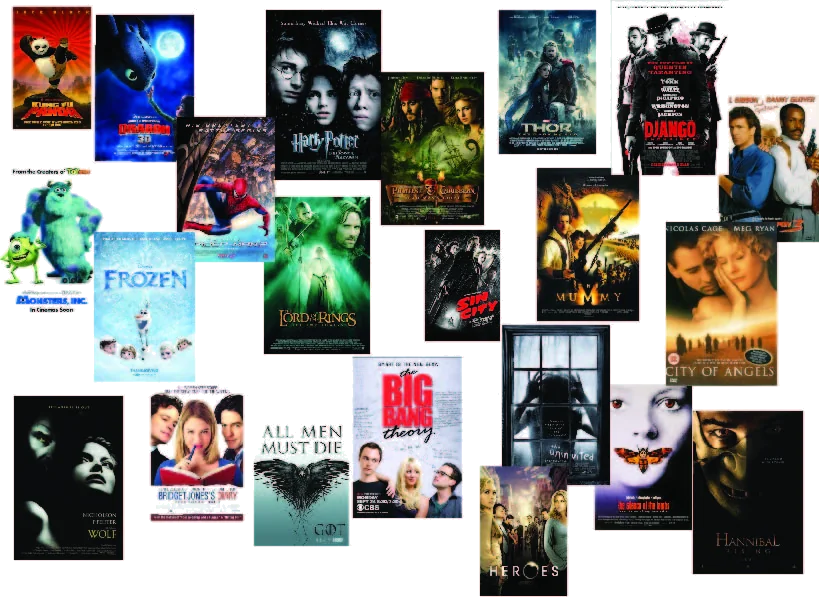
\includegraphics[width=0.8\columnwidth]{../img/movies1}}%
\only<2|handout:2>{
\textbf{but we can construct it\\[1em]}%
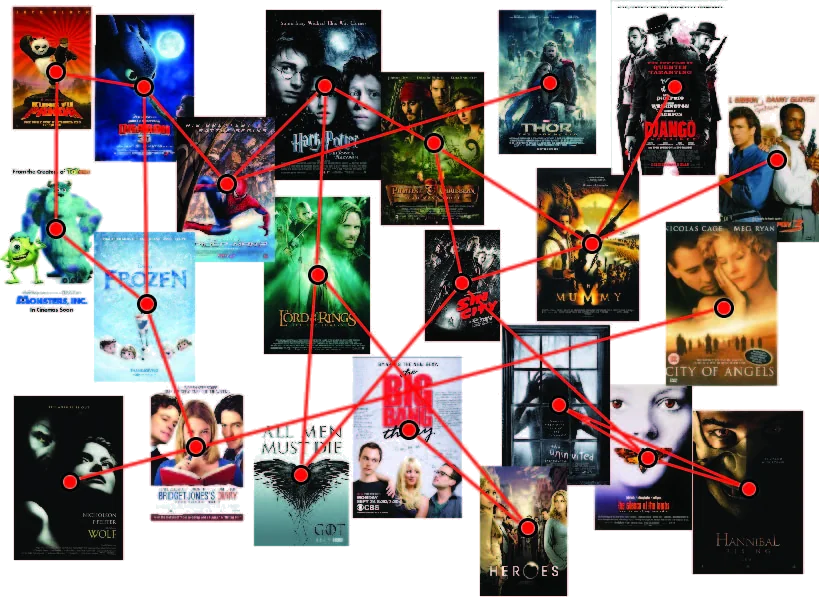
\includegraphics[width=0.8\columnwidth]{../img/movies2}}%
\only<3|handout:3>{
\textbf{and use it as an abstraction\\[1em]}%
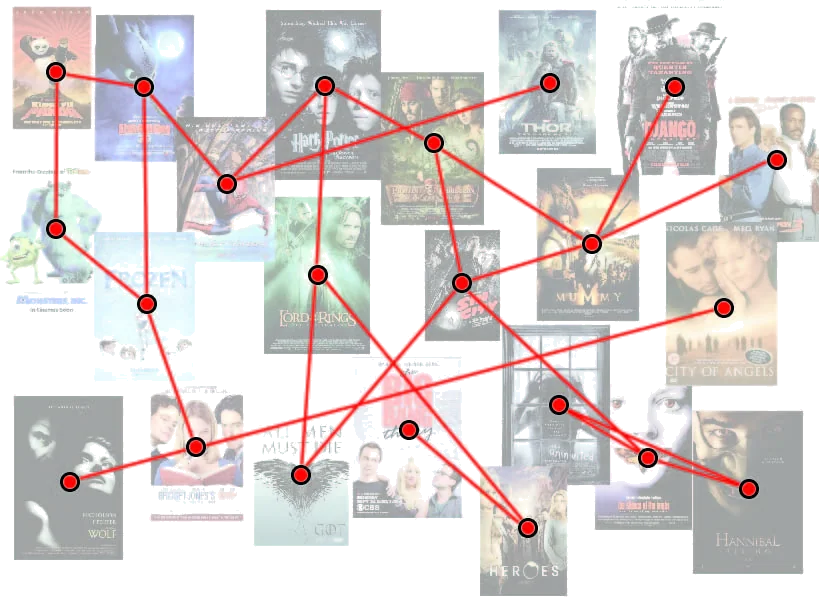
\includegraphics[width=0.8\columnwidth]{../img/movies3}}%
\end{center}
\only<4|handout:4>{
\vspace{-4em}
\begin{columns}
\begin{column}{.5\textwidth}
\begin{itemize}\addtolength{\itemsep}{1\baselineskip}
\item vision  
\item audio
\item text \pause
\item typical ML tasks 
\begin{itemize}\addtolength{\itemsep}{0.5\baselineskip}
\item semi-supervised learning  
\item spectral clustering  
\end{itemize}
\end{itemize}
\end{column}
\begin{column}{.5\textwidth}
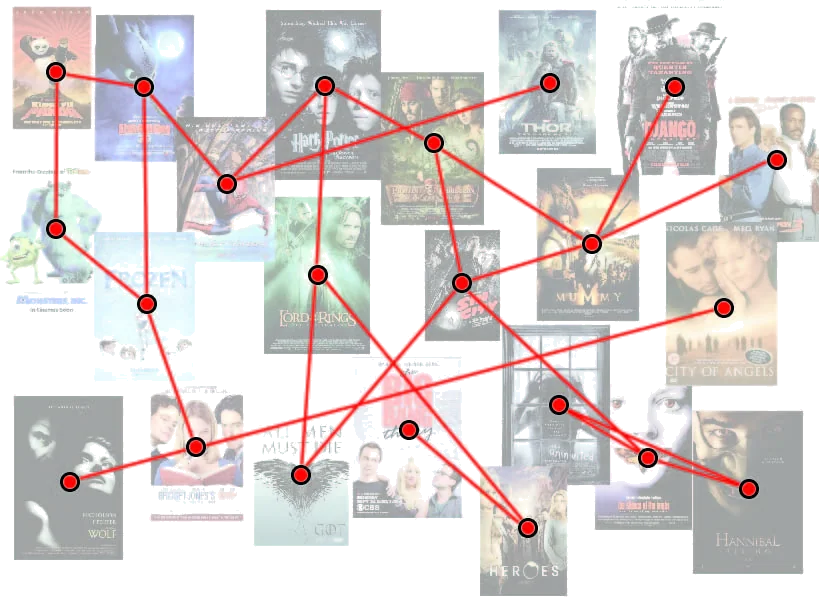
\includegraphics[width=\textwidth]{../img/movies3}\\
{\small Movie similarity} 
\end{column}
\end{columns}
}
\end{frame}
%%%%%%%%%%%%%%%%%%%%%%%%%%%%%%%%%%%%%%%%%%%%%%%%%%%%%%%%%%%%%

\begin{frame}
\frametitle{Similarity Graphs}

Input: $\bx_1, \bx_2,\bx_3, \dots, \bx_\nodes $
\begin{itemize}
\item
raw data 
\item
flat data
\item
vectorial data
\end{itemize}

\begin{center}
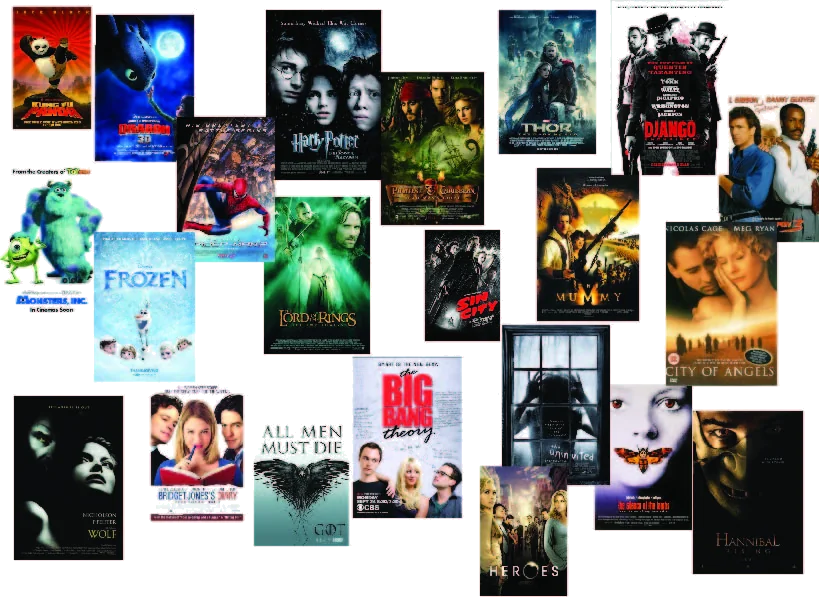
\includegraphics[width=0.6\columnwidth]{../img/movies1}
\end{center}

\end{frame}
%%%%%%%%%%%%%%%%%%%%%%%%%%%%%%%%%%%%%%%%%%%%%%%%%%%%%%%%%%%%%
%%%%%%%%%%%%%%%%%%%%%%%%%%%%%%%%%%%%%%%%%%%%%%%%%%%%%%%%%%%%%



%%%%%%%%%%%%%%%%%%%%%%%%%%%%%%%%%%%%%%%%%%%%%%%%%%%%%%%

%%%%%%%%%%%%%%%%%%%%





\MakeLastSlide
\end{document}
